%%% Local Variables: 
%%% coding: utf-8
%%% mode: latex
%%% TeX-engine: xetex
%%% End:
\documentclass[a4paper,12pt]{article} 

%\usepackage[hmargin=2.25cm, vmargin=1.5cm]{geometry} % Document margins
\usepackage[right=2cm, left=2cm,bottom=2cm,top=2cm]{geometry}

\usepackage[usenames,dvipsnames]{xcolor} % Allows the definition of hex colors
\definecolor{linkcolor}{HTML}{506266} % Blue-gray color for links
\definecolor{shade}{HTML}{F5DD9D} % Peach color for the contact information box
\definecolor{text1}{HTML}{FF0000} % Main document font color, off-black
\definecolor{headings}{HTML}{701112} % Dark red color for headings
% Other color palettes: shade=B9D7D9 and linkcolor=A40000; shade=D4D7FE and linkcolor=FF0080

\usepackage{polyglossia}
\setmainlanguage[variant=uk]{english}

\usepackage{fontspec,xltxtra,xunicode}
\defaultfontfeatures{Ligatures=TeX}
\defaultfontfeatures{Mapping=tex-text}
\setromanfont[Mapping=tex-text,SmallCapsFeatures={Scale=1.1},Numbers=OldStyle]{Optima}%{Adobe Garamond Pro} %{Hoefler Text} % Main document font
\setmonofont[Scale=0.85]{Menlo}

\newfontfamily\descitemfont{Optima}
%\newfontfamily\notefont{Lucida Handwriting}
\newcommand\descitem[1]{{\notefont #1}}
\newcommand\descitemcol[1]{{\color{headings}\descitemfont #1}}

\newenvironment{vlist}[1]{%
\begin{list}{}{%
    \settowidth{\labelwidth}{\tt #1 }     %longest label length
%    \addtolength{\labelsep}{3ex}          %extra space between lbl/txt
    \setlength{\leftmargin}{\labelwidth}  %determine leftmargin
    \addtolength{\leftmargin}{\labelsep}  %determine leftmargin
    \setlength{\parsep}{0.5ex plus 0.2ex minus 0.2ex}
    \setlength{\itemsep}{0.3ex}
    \renewcommand{\makelabel}[1]{\color{headings}\tt ##1 \color{text1}\hfill}}}%
{\end{list}}
%

\usepackage{setspace}
%\onehalfspacing
%\setstretch{1.16}%onehalf is 1.25/1.213/1.241 for 10/11/12 pt
\setstretch{1.16}

\usepackage{titlesec} % Allows creating custom \section's
% Format of the section titles
\titleformat{\section}{\color{headings}
%\scshape%
\descitemfont
\huge\raggedright}{}{0em}{}[\color{black}\titlerule]
\titlespacing{\section}{0pt}{0pt}{\baselineskip} % Spacing around titles

%\newfontfamily\subsubsectionfont[Color=MSLightBlue]{Times New Roman}
% Set formats for each heading level
%\titleformat*{\section}{\Large\bfseries\sffamily\color{MSBlue}}
%\titleformat*{\subsection}{\large\bfseries\sffamily\color{MSLightBlue}}
\titleformat*{\subsection}{\Large\color{headings}}


\usepackage{enumitem}
\SetLabelAlign{parright}{\parbox[t]{\labelwidth}{\raggedleft#1}}
\setlist[description]{style=multiline,topsep=10pt,leftmargin=2.5cm,font=\normalfont,%
    align=parright}

\newlength{\pdfwidth}
%%\setlength{\pdfwidth}{1.0\textwidth}
\setlength{\pdfwidth}{0.45\textwidth}
\newlength{\halfpage}
\setlength{\halfpage}{0.5\textwidth}
\newlength{\halfpagefig}
\setlength{\halfpagefig}{0.5\textwidth}
\addtolength{\halfpagefig}{-0.25cm}

\newcommand{\fit}[1]{\noindent\resizebox{\linewidth}{!}{#1}}

\usepackage{comment}

\begin{document}

\section*{SuperSlew}

Plugin that (a) allows you to move your plane around without actually
flying, and (b) put your plane at specific latitude and longitude coordinates.

\vspace{0.5\baselineskip}
It needs X-Plane 10.40+, and works in 32 and 64 bits, on Linux, Mac
and Windows.

\vspace{0.5\baselineskip}
The slew mode can be started and stopped in two ways. First, from the
menu, and second, by binding a key or joystick button to the custom command
defined by the plugin. The command is called
\texttt{durian/superslew/toggle}. 

\section*{Installation}

The plugin is distributed as a zip file. The \texttt{superslew}
directory and its contents, contained in the zip file, must be put in
the \texttt{Resources/plugins} directory which can be found in the
main X-Plane directory. The directory containing the plugin
\textsl{must} be called \texttt{superslew}. If installed correctly, a
new menu item called ``SuperSlew'' will appear under the Plugins menu
in X-Plane. This menu contains the following items. 

\begin{figure}[h!]%
\centering
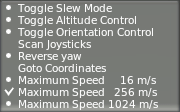
\includegraphics[scale=1]{slewstandard.png}
\label{fig:infowindow}
\end{figure}

The first menu item enables the Slew Mode. You can enable it when
flying, but when you disable the plugin again, you will continue at
the speed you had when you enabled it. This can lead to spectacular
effects if you for example rotate your plane 180 degrees, and then
continue. 

If you enable it on the ground, you can ``drive'' around, and the
plugin will keep the wheels of the plane on the ground.

If you enable the Slew Mode before going into the local map view, you
can move your plane around without crashing or ending up in the air
when you exit the map.

\subsection*{Menu Items}

\begin{vlist}{w}

\item[Toggle Slew Mode] Switches the slew mode on or
off. When enabled, a small windows containing information is shown in
the bottow right corner of the screen. 

\item[Toggle Altitude Control] Enabling altitude control makes the
  plane move up or down when you move the joystick to the right or
  left. Note that you can not go below the altitude you were when you
  enabled the SuperSlew Mode. This is to prevent disappearing under
  ground. There is more information on how to control the plane in the
  next section.

\item[Toggle Orientation Control] This mode lets you control the
  orientation of the plane. There is more information on how to
  control the plane in the next section.

\item[Scan Joysticks] Rescans the joysticks connected to the computer.

\item[Reverse yaw] Reverses the orientation of the yaw (heading) control.

\item[Goto Coordinates] Shows a dialog box in which you can enter a
  latitude and longitude. Pressing goto will put your plane at the
  specified coordinates.
\begin{figure}[h!]%
\centering
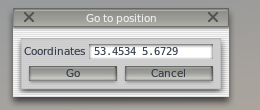
\includegraphics[scale=1]{slewgoto.png}
\label{fig:infowindow}
\end{figure}
Use a minus sign for coordinates to the west of Greenwhich or south
of the equator. The coordinates need to be in decimal format, and the need
to be seperated by a single space only. The screen shot shows a
position in The Netherlands.

\item[Maximum Speed 16 m/s] Full throttle will move your plane at this
  speed. Different speed settings exists to allow better control. The
  slowest setting is goot for taxiiing around the airport, with a
  maximum speed of 31 knots.

\item[Maximum Speed 256 m/s] Full throttle will move your plane at this
  speed. 

\item[Maximum Speed 1024 m/s] Full throttle will move your plane at this
  speed. Moving very fast can cause the loading of the scenery to lag
  behind. It will catch up again when you are stationary.

\end{vlist}{}
\section*{Controls}

%explain modes first, and what is standard mode
When you start the plugin for the first time, the plane can be moved
around with the joystick and/or pedals. Moving the stick forward or
backward will move the plane forward of backward. Moving the stick to
the right or left moves your plane to the right or left.  The speed at
which you move is controlled by the throttle.

\vspace{0.5\baselineskip}
You can rotate the plane with the pedals (or twist grip on your
joystick). Speed of rotation is controlled by how much you move the
pedals or stick.

%\begin{figure}[h!]%
%\centering
%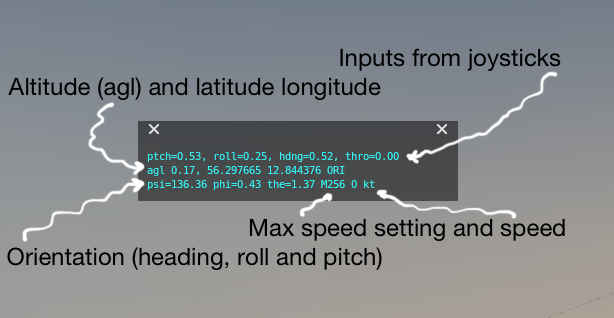
\includegraphics[width=1.0\textwidth]{infowindow.png}
%\label{fig:infowindow}
%\end{figure}

\subsection*{Altitude control}

\begin{figure}[h!]%
\centering
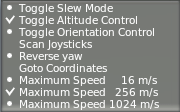
\includegraphics[scale=1]{slewaltitude.png}
\label{fig:infowindow}
\end{figure}

Moving the stick to the right or left moves your plane to the right or
left. If you select the ``Altitude Mode'' from the menu, your plane
will be moved up or down instead. You can not go below the altitude
your are at when you enable the plugin. This is to prevent
disappearing under ground. As a consequence, you can not start the
Slew Mode in the air and put your plane down on the ground.

\vspace{0.5\baselineskip}
You can rotate the plane with the pedals (or twist grip on your
joystick). Speed of rotation is controlled by how much you move the
pedals or stick.

\vspace{0.5\baselineskip}
If you switch to ``Orientation Mode'', you can change the pitch and
roll with the joystick. The pedals still change the rotation. This
mode disables the two other modes, so you have to disable it if you
want to move position again.

\begin{figure}[h!]%
\centering
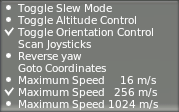
\includegraphics[scale=1]{sleworientation.png}
\label{fig:infowindow}
\end{figure}

\vspace{0.5\baselineskip}
This readme is for version 0.93. 

\vspace{0.5\baselineskip} {\color{text1}This program is shareware. You may try
  it, but if you keep on using it you are encouraged to make a small
  donation. May not be re-distributed, sold or used for commercial
  purposes without explicit permission.}

\end{document}
